\newpage
\subsection{Caso d'uso UC4: Logout}
	\label{UC4}
	\begin{figure}[ht]
		\centering
			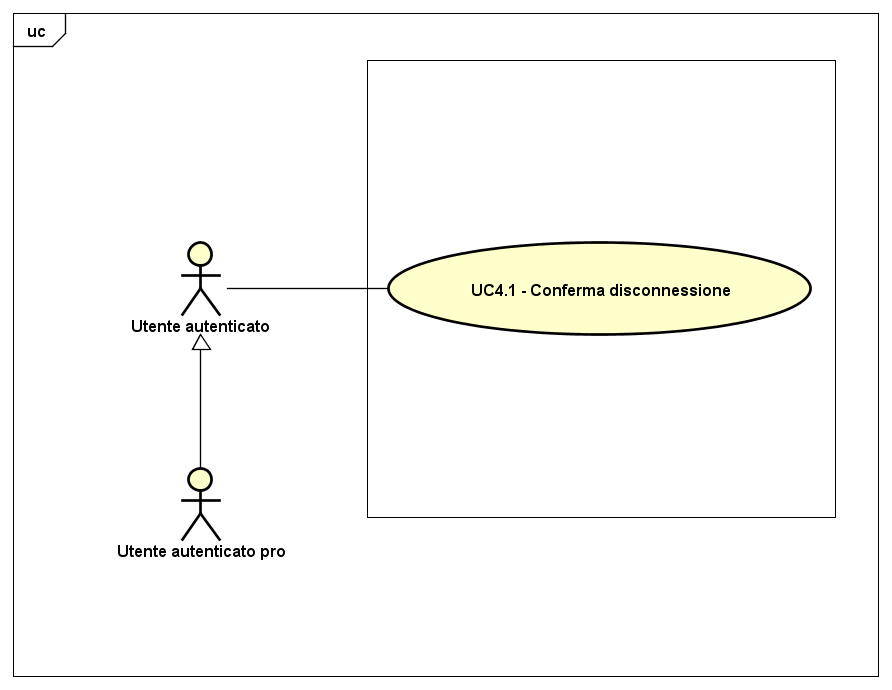
\includegraphics[scale=0.5,keepaspectratio]{UML/UC4.png}
		\caption{UC4: Logout}
	\end{figure}
	\FloatBarrier
	\begin{itemize}
		\item
			\textbf{Attori}: utente autenticato, utente autenticato pro;
		\item		
			\textbf{Descrizione}: l'attore può terminare la sua sessione, uscendo dalla sua area riservata;
		\item
			\textbf{Precondizione}: il sistema presenta la funzionalità utile all'attore per uscire dalla sua area riservata;
		\item
			\textbf{Postcondizione}: l'attore non è autenticato presso il sistema;
		\item
			\textbf{Scenario principale}: l'attore conferma la disconnessione (UC4.1).
	\end{itemize}

\subsubsection{Caso d'uso UC4.1: Conferma disconnessione}
	\begin{itemize}
		\item
			\textbf{Attori}: utente autenticato, utente autenticato pro;
		\item
			\textbf{Descrizione}: l'attore può confermare di voler effettuare il logout;
 		\item
			\textbf{Precondizione}: il sistema ha ricevuto la richiesta di logout da parte dell'attore;
		\item
			\textbf{Postcondizione}: il sistema conferma all'attore l'uscita dalla sua area riservata;
		\item
			\textbf{Scenario principale}: l'attore conferma di voler effettuare il logout.
	\end{itemize}		
	